\documentclass[conference]{IEEEtran}
\IEEEoverridecommandlockouts
% The preceding line is only needed to identify funding in the first footnote. If that is unneeded, please comment it out.
\usepackage{amsmath,amsthm,amssymb} %modos matemáticos y  simbolos
\usepackage{latexsym,amsfonts} %simbolos matematicos
\usepackage{cancel} %hacer la linea que cancela las ecuaciones
\usepackage[spanish, es-noshorthands]{babel} %comandos en español y cambia el cuadro por la tabla
\decimalpoint %cambia las comas por puntos decimal
\usepackage[utf8]{inputenc} %caracteristicas del español
\usepackage{physics} %Simbolos fisicos
\usepackage{array} %mejores formatos de tabla
\parindent =0cm %sangria 
\usepackage{algorithmic}
\usepackage{graphicx}
\usepackage{textcomp}
\usepackage{xcolor}
\usepackage{mathtools} 
\usepackage[framemethod=TikZ]{mdframed}%Entornos talegas
\usepackage[colorlinks = true,
			linkcolor = blue,
			citecolor = black,
			urlcolor = blue]{hyperref}%formato de los links y URL's
\usepackage{multicol} %varias columnas
\usepackage{enumerate} %enumeraciones
\usepackage{pgf,tikz,pgfplots} %documentos en formato tikz
\usepackage{mathrsfs} %letras chingonas (transformada de laplace)
\usepackage{subfigure} %varias figuras seguidas
\usepackage{tabulary}
\usepackage{multirow} %ocupar varias filas en una tabla
\usepackage{fancybox} %recuadros talegas
\usepackage{float} %ubicar graficas
\usepackage{color}
\usepackage{comment}
\usepackage{stackrel}
\usepackage{calligra}
\usepackage{lipsum}
\usepackage{cite}

\newcommand{\R}{\mathbb{R}}
%%%%%%%%%%%%%%%%%%%%%%%%%%%%%%%%%%%%%%%%%%%%%%%%%%%%%%
\def\BibTeX{{\rm B\kern-.05em{\sc i\kern-.025em b}\kern-.08em
    T\kern-.1667em\lower.7ex\hbox{E}\kern-.125emX}}
\begin{document}

\title{Péndulo Simple\\
{\footnotesize \scshape{Reporte 1}}
}

\author{\IEEEauthorblockN{1\textsuperscript{sd} Diego Sarceño Ramírez}
\IEEEauthorblockA{\textit{201900109} \\
}
}

\maketitle

\begin{abstract}
    En este trabajo se encuentra el valor de la gravedad por medio de medición del tiempo de cierta cantidad de oscilaciones. A los valores encontrados se le añade el tiempo de reacción del experimentador para obtener una mejor aproximación. Además, se utiliza un software para verificar las relaciones teóricas ya conocidas, por medio de gráficas realizadas con \textit{Gnuplot}\footnote{El código puede ser encontrado en un repositorio \href{https://github.com/DSarceno/Semestre5/tree/main/ReduccionDatos/Reporte1/graficas}{Github} }.
\end{abstract}

\begin{IEEEkeywords}
    Péndulo simple, periodo.
\end{IEEEkeywords}

\section{Objetivos}

\subsection{General}
    \begin{enumerate}[1.]
        \item Determinar el valor de la gravedad por medio del experimento del péndulo simple.
    \end{enumerate}
\subsection{Específicos}
    \begin{enumerate}[a)]
        \item Utilizar el tiempo de reacción para obtener medidas mejor aproximadas para el valor de la gravedad.
        \item Encontrar el número de oscilaciones apto para disminuir en cierto factor el error relativo de la gravedad.
        \item Comparar y ampliar los resultados utilizando datos obtenidos en un sofware web.
    \end{enumerate}

%\section{Introducción}
    

\section{Marco Teórico}
    El diseño del péndulo simple es muy sencillo, el análisis de fuerzas realizado en coordenadas polares, es
    \begin{align}
    	F_{\theta} = -mg\theta = -\frac{mg}{L} x, \label{omega}
    \end{align}
    de modo que $\omega = \sqrt{\flatfrac{g}{l}}$\footnote{Ecuación $14.32$ de \cite{b2}}. Además, la relación entre $\omega$ y el periodo es $\omega = \flatfrac{2\pi}{T}$.
    
\section{Diseño Experimental}
    El péndulo simple, utiliza pocos materiales:
    \begin{itemize}
    	\item Cuerda/hilo resistente y no estirable.
    	\item Pivote (en este caso fue una escoba).
    	\item Transportador.
    	\item Masa (en este caso, pieza de madera).
    \end{itemize}
    El procedimiento utilizado:
    \begin{enumerate}
    	\item Armar el péndulo colgando del pivote el hilo con la masa amarrada al otro extremo.
    	\item Colocar el transportador de modo que su centro este en el nudo del hilo con el pivote.
    \end{enumerate}
    Resultado visual:
    \begin{figure}[H]
    	\centering
    	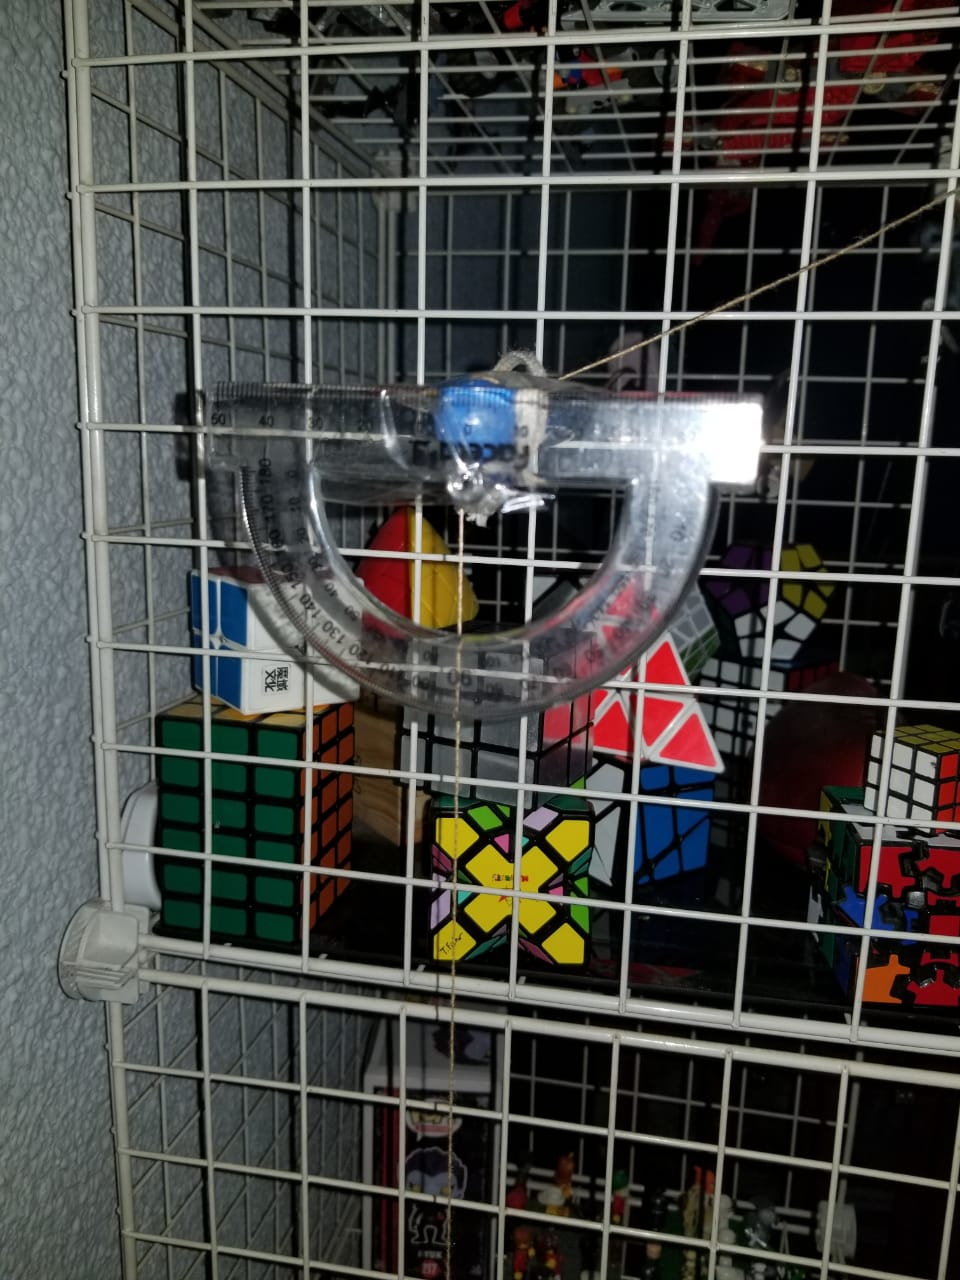
\includegraphics[scale=0.15]{fotos/1.jpeg}
    	\caption{Vértice con el transportador. (El fondo utilizado no alcanzó para la parte superior del experimento)}
    \end{figure}
    \begin{figure}[H]
    	\centering
    	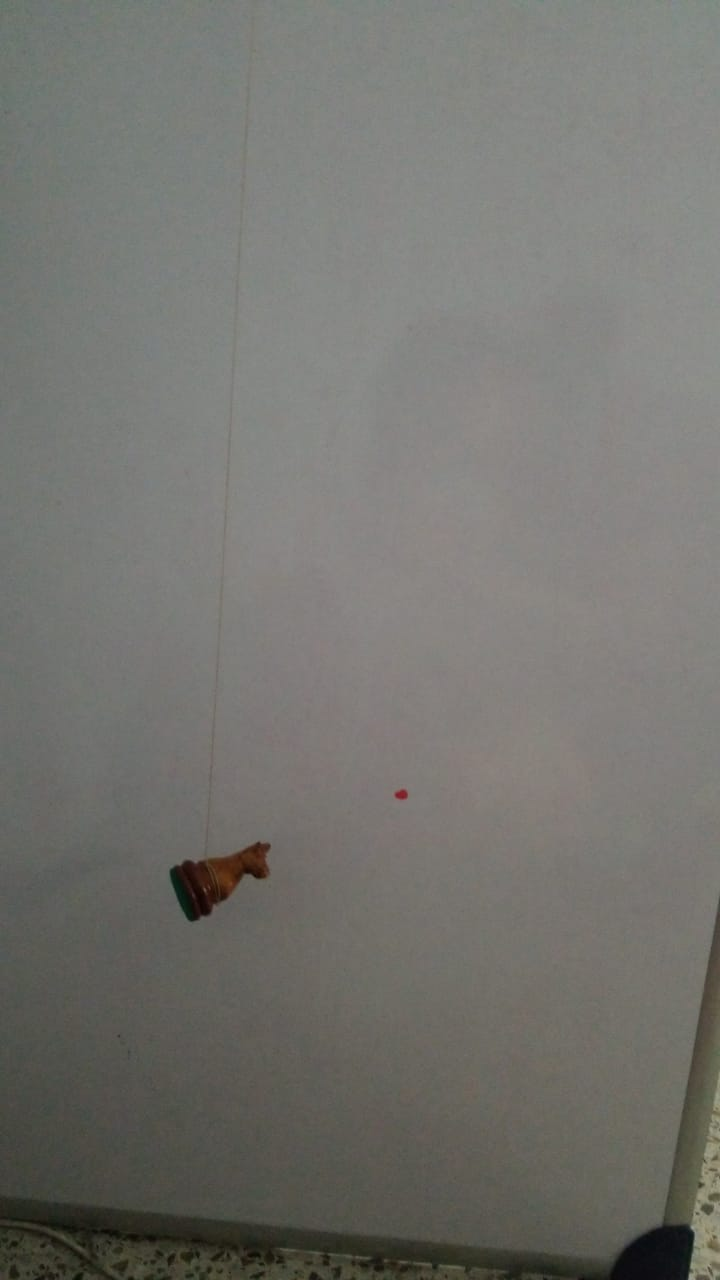
\includegraphics[scale=0.15]{fotos/2.jpeg}
    	\caption{Parte baja del sistema, se utilizó una masa lo suficientemente grande para generar el movimiento de oscilación bastante constante y no tan grande como para generar oscilaciones verticales o romper el hilo.}
    \end{figure}

    
\section{Resultados}
    Para calcular la gravedad, se tomaron varias medidas del tiempo de $5$ oscilaciones para tener varias y escojer la más cercana al valor esperado: (Longitud de la cuerda $L = 98.0 \pm 0.1 cm = 0.980 \pm 0.001 m$)
    \begin{table}[H]
    	\centering
    	\caption{Gravedad (Sin tiempo de Reacción)}
    	\begin{tabular}{||c||c|c|c||}
    		\hline
    		\hline
    			& $t\pm \delta t [s]$ & $T \pm \delta T [s]$ & $g \pm \delta g [m/s^2]$ \\
    		\hline
    		\hline
    			& $9.95 \pm 0.01$ & $(1990 \pm 2) \times 10^{-3}$ & $9.77 \pm  0.02$ \\
    			
    			& $9.88 \pm 0.01$ & $(1976 \pm 2) \times 10^{-3}$ & $9.91 \pm  0.02$ \\
    			& $10.01 \pm 0.01$ & $(2002 \pm 2) \times 10^{-3}$ & $9.65 \pm  0.02$ \\
    			$\to$ & $9.93 \pm 0.01$ & $(1986 \pm 2) \times 10^{-3}$ & $9.81 \pm  0.02$ \\
    			& $9.84 \pm 0.01$ & $(1968 \pm 2) \times 10^{-3}$ & $9.99 \pm  0.02$ \\		
    		\hline
    		\hline
    	\end{tabular}
    	\label{tab:res1}
    \end{table}
    
    Las expresiónes teóricas utilizadas para el cálculo de la gravedad y su incerteza (asumiendo variables independientes aleatorias), son \eqref{omega} y:
    \begin{align*}
    	\frac{\delta g}{g} &= \sqrt{\qty(\frac{\delta L}{L})^2 + \qty(\frac{2\delta T}{T})^2}
    \end{align*}
    
    El tiempo de reacción utilizando las $5$ alturas encontradas y \eqref{tr}
    \begin{align*}
    	\left.\begin{array}{c}
    		h_1 = 4.5 cm = 0.045 m \\
    		h_2 = 14.3 cm = 0.143 m \\
    		h_3 = 8.5 cm = 0.085 m \\
    		h_4 = 13 cm = 0.13 m \\
    		h_5 = 9 cm = 0.09 m
    	\end{array}\right\} \Rightarrow
    	t_R  = 0.14 s
    \end{align*}
    Sumando esto a la incerteza del tiempo medido. Tomando únicamente el valor más aproximado al valor real. Por lo que
    \begin{table}[H]
    	\centering
    	\caption{Gravedad}
    	\begin{tabular}{||c||c|c|c||}
    		\hline
    		\hline
    			& $t\pm \delta t [s]$ & $T \pm \delta T [s]$ & $g \pm \delta g [m/s^2]$ \\
    		\hline
    			$\to$ & $9.93 \pm 0.15$ & $1.99 \pm 0.03$ & $9.81 \pm  0.15$ \\
    		\hline
    		\hline
    	\end{tabular}
    	\label{tab:res2}
    \end{table}
    
    Utilizando \eqref{N} se tiene que el número de oscilaciónes requerido para que el error relativo de la gravedad sea igual que el error relativo de la longitud es (tomando la incerteza del tiempo con el tiempo de reacción) es de $N = 147.7 \approx 148$. Lo que da
    \begin{table}[H]
    	\centering
    	\caption{Gravedad ($148$ oscilaciones)}
    	\begin{tabular}{||c||c|c|c||}
    		\hline
    		\hline
    			& $t\pm \delta t [s]$ & $T \pm \delta T [s]$ & $g \pm \delta g [m/s^2]$ \\
    		\hline
    			$\to$ & $296.84 \pm 0.15$ & $2.0057 \pm 0.001$ & $9.67 \pm  0.01$ \\
    		\hline
    		\hline
    	\end{tabular}
    	\label{tab:res2}
    \end{table}
    Lo que da un error relativo de $\flatfrac{\delta g}{g} = 1.15\times 10^{-3}$, muy parecido al error relativo de la longitud $\flatfrac{\delta L}{L} = 1.02\times 10^{-3}$. \\
    
    Utilizando \cite{b1} se obtuvieron los siguientes resultados:
    \begin{table}[H]
    	\centering
    	\caption{Longitud fija en $1m$.}
    	\begin{tabular}{||c|c|c||}
    		\hline
    		\hline
				Masas & Tiempo $[s]$ $10$ Oscilaciones & Tiempo $[s]$ $1$ Oscilación \\
    		\hline
    		\hline
    			$100$ & $20$ & $2$ \\
    			$300$ & $20$ & $2$ \\
    			$500$ & $20$ & $2$ \\
    		\hline
    		\hline
    	\end{tabular}
    \end{table}
    
    \begin{figure}[H]
    	\centering
    	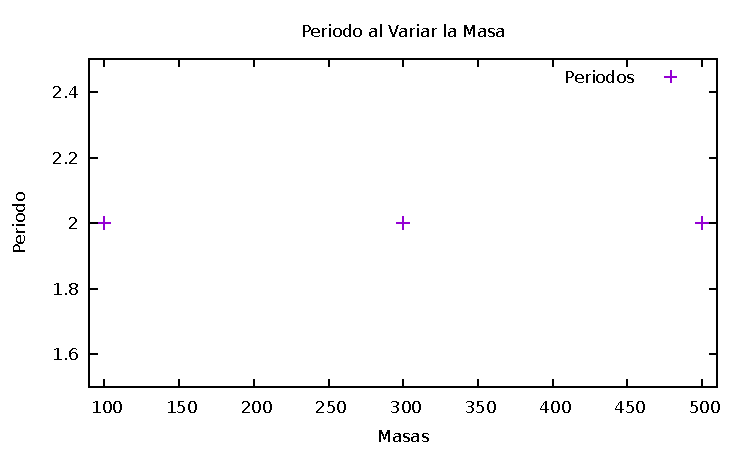
\includegraphics[scale=0.5]{graficas/masas.pdf}
    	\caption{Relación entre la variación en la masa y el tiempo de oscilación.}
    \end{figure}
    
    
    
    \begin{table}[H]
    	\centering
    	\caption{Variando la Longitud.}
    	\begin{tabular}{||c|c|c||}
    		\hline
    		\hline
				Longitudes $[m]$ & Tiempo $[s]$ $10$ Osc. & Tiempo $[s]$ $1$ Osc. \\
    		\hline
    		\hline
    			$0.5$ & $14$ & $1.4$ \\
    			$1$ & $20$ & $2$ \\
    			$2$ & $28$ & $2.8$ \\
    		\hline
    		\hline
    	\end{tabular}
    \end{table}
    
    \begin{figure}[H]
    	\centering
    	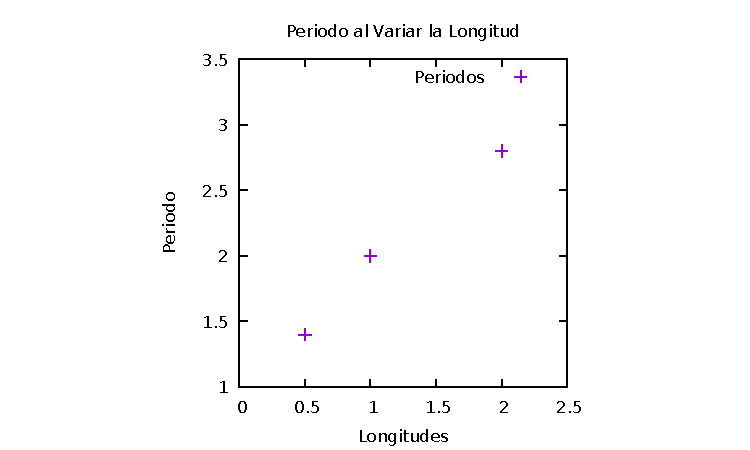
\includegraphics[scale=0.6]{graficas/longitudes.pdf}
    	\caption{Relación entre la variación en la longitud y el tiempo de oscilación.}
    \end{figure}
    
    
    
    \begin{table}[H]
    	\centering
    	\caption{Variando el Ángulo.}
    	\begin{tabular}{||c|c|c||}
    		\hline
    		\hline
				Ángulos (Grados) & Tiempo $[s]$ $10$ Osc. & Tiempo $[s]$ $1$ Osc. \\
    		\hline
    		\hline
    			$5$ & $20$ & $2$ \\
    			$10$ & $20$ & $2$ \\
    			$20$ & $19$ & $1.9$ \\
    		\hline
    		\hline
    	\end{tabular}
    \end{table}
    
    \begin{figure}[H]
    	\centering
    	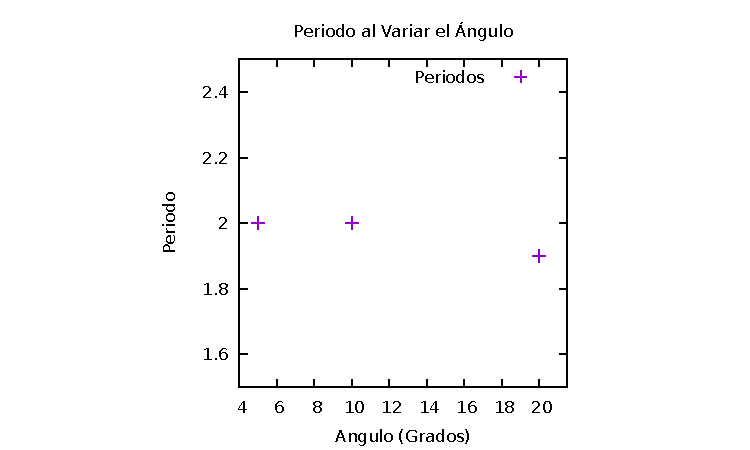
\includegraphics[scale=0.6]{graficas/angulos.pdf}
    	\caption{Relación entre la variación en el ángulo y el tiempo de oscilación. Las gráficas fueron realizadas con un código hecho en \textit{Gnuplot}.}
    \end{figure}
    
    
    
\section{Discución de Resultados}
    \begin{enumerate}
        \item Se realizaron varias mediciones de tiempo para tener una aproximación bastante correcta y en base a dicha aproximación utilizar el tiempo de reacción para tener la medida más real. La aproximación hecha de la gravedad tiene un error absoluto del $0.1\%$ lo que valida la medida.
        \item El número relativo de la gravedad se aproxima al error relativo de la longitud, la pequeña diferencia encontrada es debida a la pérdida de enrgía al ser tantas oscilaciones; además, del tiempo de reacción que se añade a la incerteza de la medida. A pesar de ello, el error relativo se aproxima.
        \item Los resultados obtenidos en el software web son aproximados a los modelos teóricos. Para la variación de la longitud, se cumple la relación obtenida de \eqref{omega}, la cual es una dependencia de raíz cuadrática. Gráficamente se sustentan los resultados con la teoría. El medidor de tiempo utilizado es el que proporciona la página, puesto que si se utiliza un medidor externo se añadirían aún más factores perjudiciales al resultado.
    \end{enumerate}
    
\section{Conclusiones}
    \begin{enumerate}
        \item La inclusión del tiempo de reacción vuelve hace que la medida sea más aceptable en cuanto a su incerteza se refiere. Además, la aproximación hecha de la gravedad difiere en un porcentaje despreciable del valor teórico más aceptado.
        \item Al aumentar el número de oscilaciones, teóricamente, disminuye el error relativo hasta ser igual al error relativo de la longitud; sin embargo, la pérdida de energía y el tiempo de reacción, simplemente aproximan este resultado.
        \item Los resultados obtenidos en el software web, son consistentes con la teoría vista en \cite{b2}. 
    \end{enumerate}



%\section{Recomendaciones}

\section{Anexos}
    Fórmula del promedio/media de cierta cantidad de medidas:
    \begin{align}
	 	\bar{h} &= \frac{1}{n} \sum_{i=1} ^n h_i .   	\label{mean}
    \end{align}
    Además, por cinemática (ignorando la resistencia del aire) se tiene que el tiempo de reacción es
    \begin{align}
    	t_R &= \sqrt{\frac{2\bar{h}}{g}}, \label{tr}
    \end{align}
    es válido utilizar la gravedad aqui, puesto que este es considerado un experimento aparte al realizado en el laboratorio. \\
    Para encontrar el número de oscilaciones, se utiliza la ecuación dada en clase
    \begin{align}
    	N = \frac{2L\delta t}{\delta L T}. \label{N}
    \end{align}
    
    
\begin{thebibliography}{00}
\bibitem{b1} Tema Fantástico, S.A., \textit{Laboratorio Virtual} \href{https://labovirtual.blogspot.com/search/label/El\%20p\%C3\%A9ndulo\%20simple}{URL}
\bibitem{b2} Sears y Zemansky, \textit{Física Universitaria}, 13ed. México: $2013$.
\end{thebibliography}

\end{document}
